%----------------------------------------------------%
%               PROCESAMIENTO DE DATOS               %
%----------------------------------------------------%

\pagestyle{fancy}

\chapter{Procesamiento y Resultados}
\label{procesamiento_datos}

En el presente capítulo, el penúltimo del documento, se analiza el código implementado para materializar las consultas definidas en el apartado \ref*{definicion_consultas}. A su vez, se publican los resultados obtenidos mediante la ejecución de dichos códigos y a la postre se analizan las diferencias existentes entre ambos entornos.

\section{Procesamiento de datos}

El código ejecutado para procesar los datos almacenados en ambos entornos es diametralmente opuesto.\\

Por un lado, en el entorno centralizado, se hace uso de SQL, un lenguaje de consultas nativo y totalmente estandarizado desde hace décadas. Ofrece la posibilidad de recuperar cualquier subconjunto de datos entre los almacenados utilizando una sintaxis relativamente sencilla.\\

Por el otro, en el entorno distribuido, el proceso se complica de sobremanera ya que es necesario lidiar con varias tecnologías a la vez y tener en cuenta las restricciones que cada una de ellas presenta. Ello implica la conveniencia de utilizar una capa de abstracción superior que unifique el funcionamiento de ambas tecnologías, como por ejemplo un conector, lo cual genera la necesidad de conocer distintas sintaxis y además imposibilita el saber qué es lo que se acaba ejecutando en las capas inferiores.\\

\subsection{Entorno centralizado}
 
\subsubsection[]{MYSQL01}

\begin{figure}[h]
	\centering
	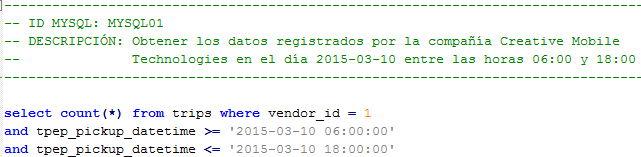
\includegraphics[width=1\textwidth]{Ilustraciones/MYSQL01.png}
\end{figure}

\subsubsection[]{MYSQL02}

\begin{figure}[h]
	\centering
	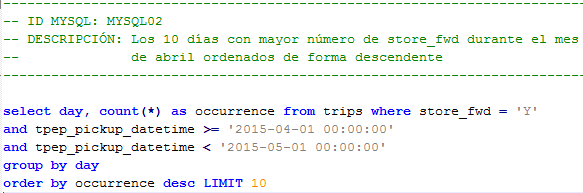
\includegraphics[width=1\textwidth]{Ilustraciones/MYSQL02.png}
\end{figure}

\clearpage

\subsubsection[]{MYSQL03}

\begin{figure}[h]
	\centering
	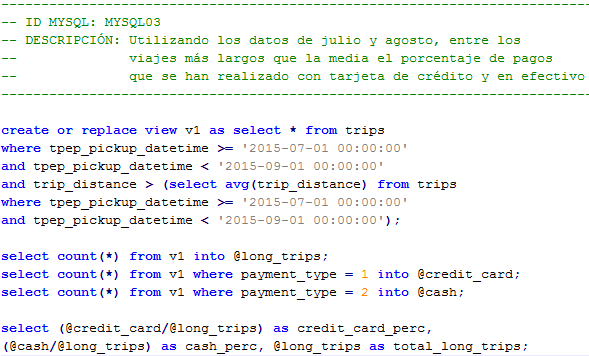
\includegraphics[width=1\textwidth]{Ilustraciones/MYSQL03.png}
\end{figure}

\subsubsection[]{MYSQL04}

\begin{figure}[h]
	\centering
	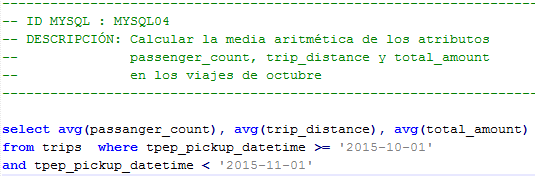
\includegraphics[width=1\textwidth]{Ilustraciones/MYSQL04.png}
\end{figure}

\clearpage

\subsection{Entorno distribuido}

Debido a la vasta sintaxis que se necesita para los preparativos de la ejecucion de una consulta dedefinir una consulta que interaccione tanto con Cassandra como con Spark, se ha decidido presentar

// saque a la luz los aspectos mas relevantes

// Ademas se intenta explicar resumidamente los detalles mas reseñables del codigo publicado

\subsubsection[]{CLU01}

Representa una consulta típica en Cassandra. En ella se especifican los atributos 'vendor\_id' y 'dia' que componen la Partition Key de la tabla donde están almacenados los datos y además mediante el clustering column 'tpep\_pickup\_datetime' se filtran los registro de dicha particion.

\begin{figure}[h]
	\centering
	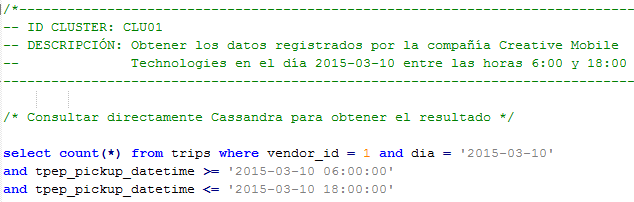
\includegraphics[width=1\textwidth]{Ilustraciones/CLU01.png}
\end{figure}

\clearpage

\subsubsection[]{CLU02}

Ante la imposibilidad de filtrar utilizando el atributo 'store\_fwd' debido a las restricciones que presenta la tabla diseñada, es necesario echar mano de Spark. Esta tecnología permite almacenar los registros en memoria RAM y computar operaciones que en Cassandra no son posibles. 

\begin{figure}[h]
	\centering
	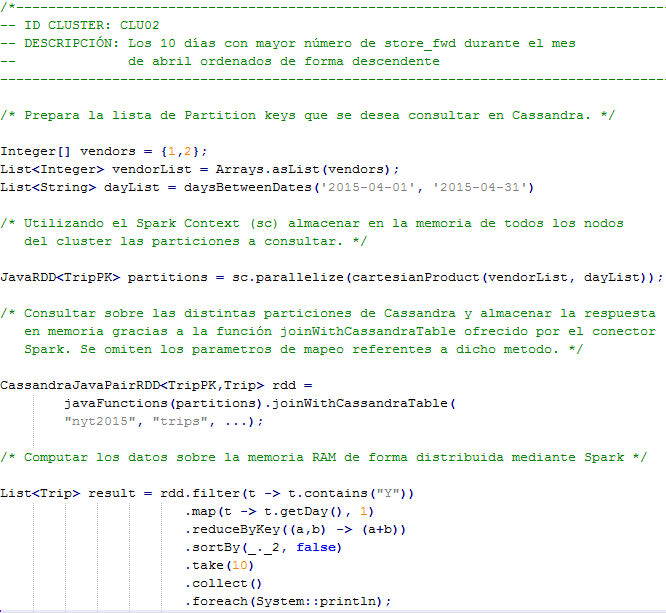
\includegraphics[width=1\textwidth]{Ilustraciones/CLU02.png}
\end{figure}

\clearpage

\subsubsection[]{CLU03}

Cache en operaciones que iteran reiteradamente sobre una misma RDD en memoria. Explicar las ventajas (indica que ya estan cargados y ahorra ese trabajo)

\begin{figure}[h]
	\centering
	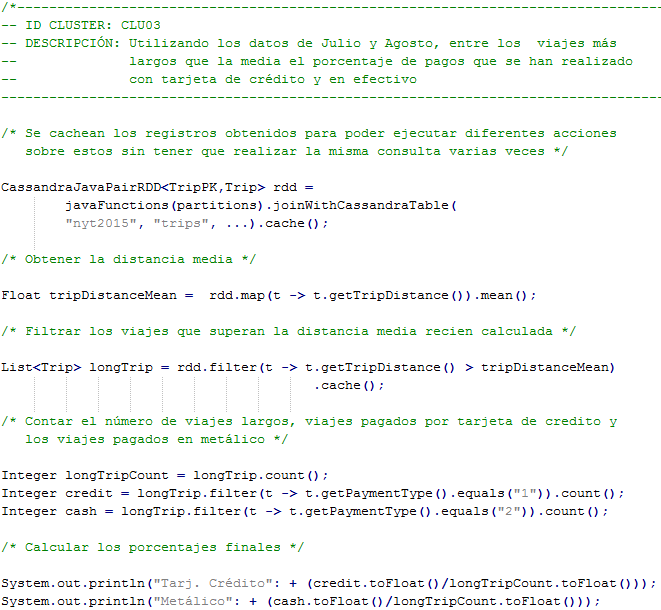
\includegraphics[width=1\textwidth]{Ilustraciones/CLU03.png}
\end{figure}

\clearpage

\subsubsection[]{CLU04}

Consulta que imita al proceso Cálculo de Indicadores de forma simplificada

se podrian almacenar las medias de un dia en una tabla aparte y partiendo de ahi calcular las medias de cada y mes y las anuales

\begin{figure}[h]
	\centering
	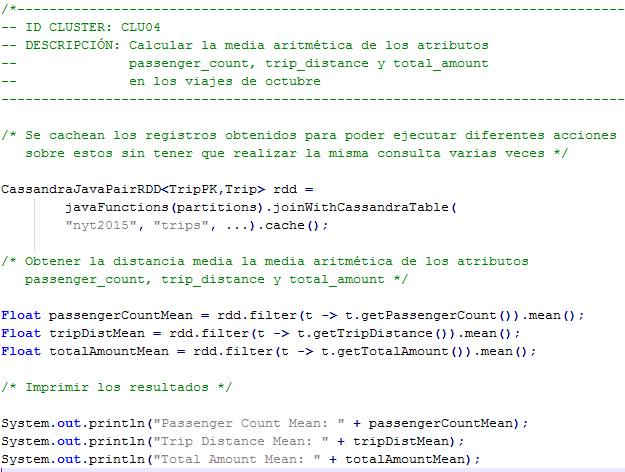
\includegraphics[width=1\textwidth]{Ilustraciones/CLU04.png}
\end{figure}

\clearpage

\section{Resultados}

Una vez habiendo conocido los entresijos de las consultas diseñadas para probar el rendimiento de los entornos confeccionados, es hora de poner el broche final al capítulo presentando los resultados obtenidos a consecuencia su ejecución.

Aprovechando que para realizar las consultas ha sido necesario insertar los registros en las respectivas bases de datos, se ha medido el ratio de inserciones por segundo ofrecido tanto por MySQL Server como por Cassandra.\\ 

\subsection{Inserciones}

Al contrario de lo que se podría esperar a inicialmente\cite{rabl2012solving}, MySQL Server empieza insertando los primeros registros con un ratio de escritura por segundo 15 veces superior al de Cassandra. No obstante, su rendimiento empieza a decaer de forma exponencial a medida que se van almacenando más registros, llegando a rendir a la par de Cassandra. Cassandra, no obstante,  demuestra ser capaz de mantener un ritmo de inserción constante
 
 \begin{figure}[h]
 	\centering
 	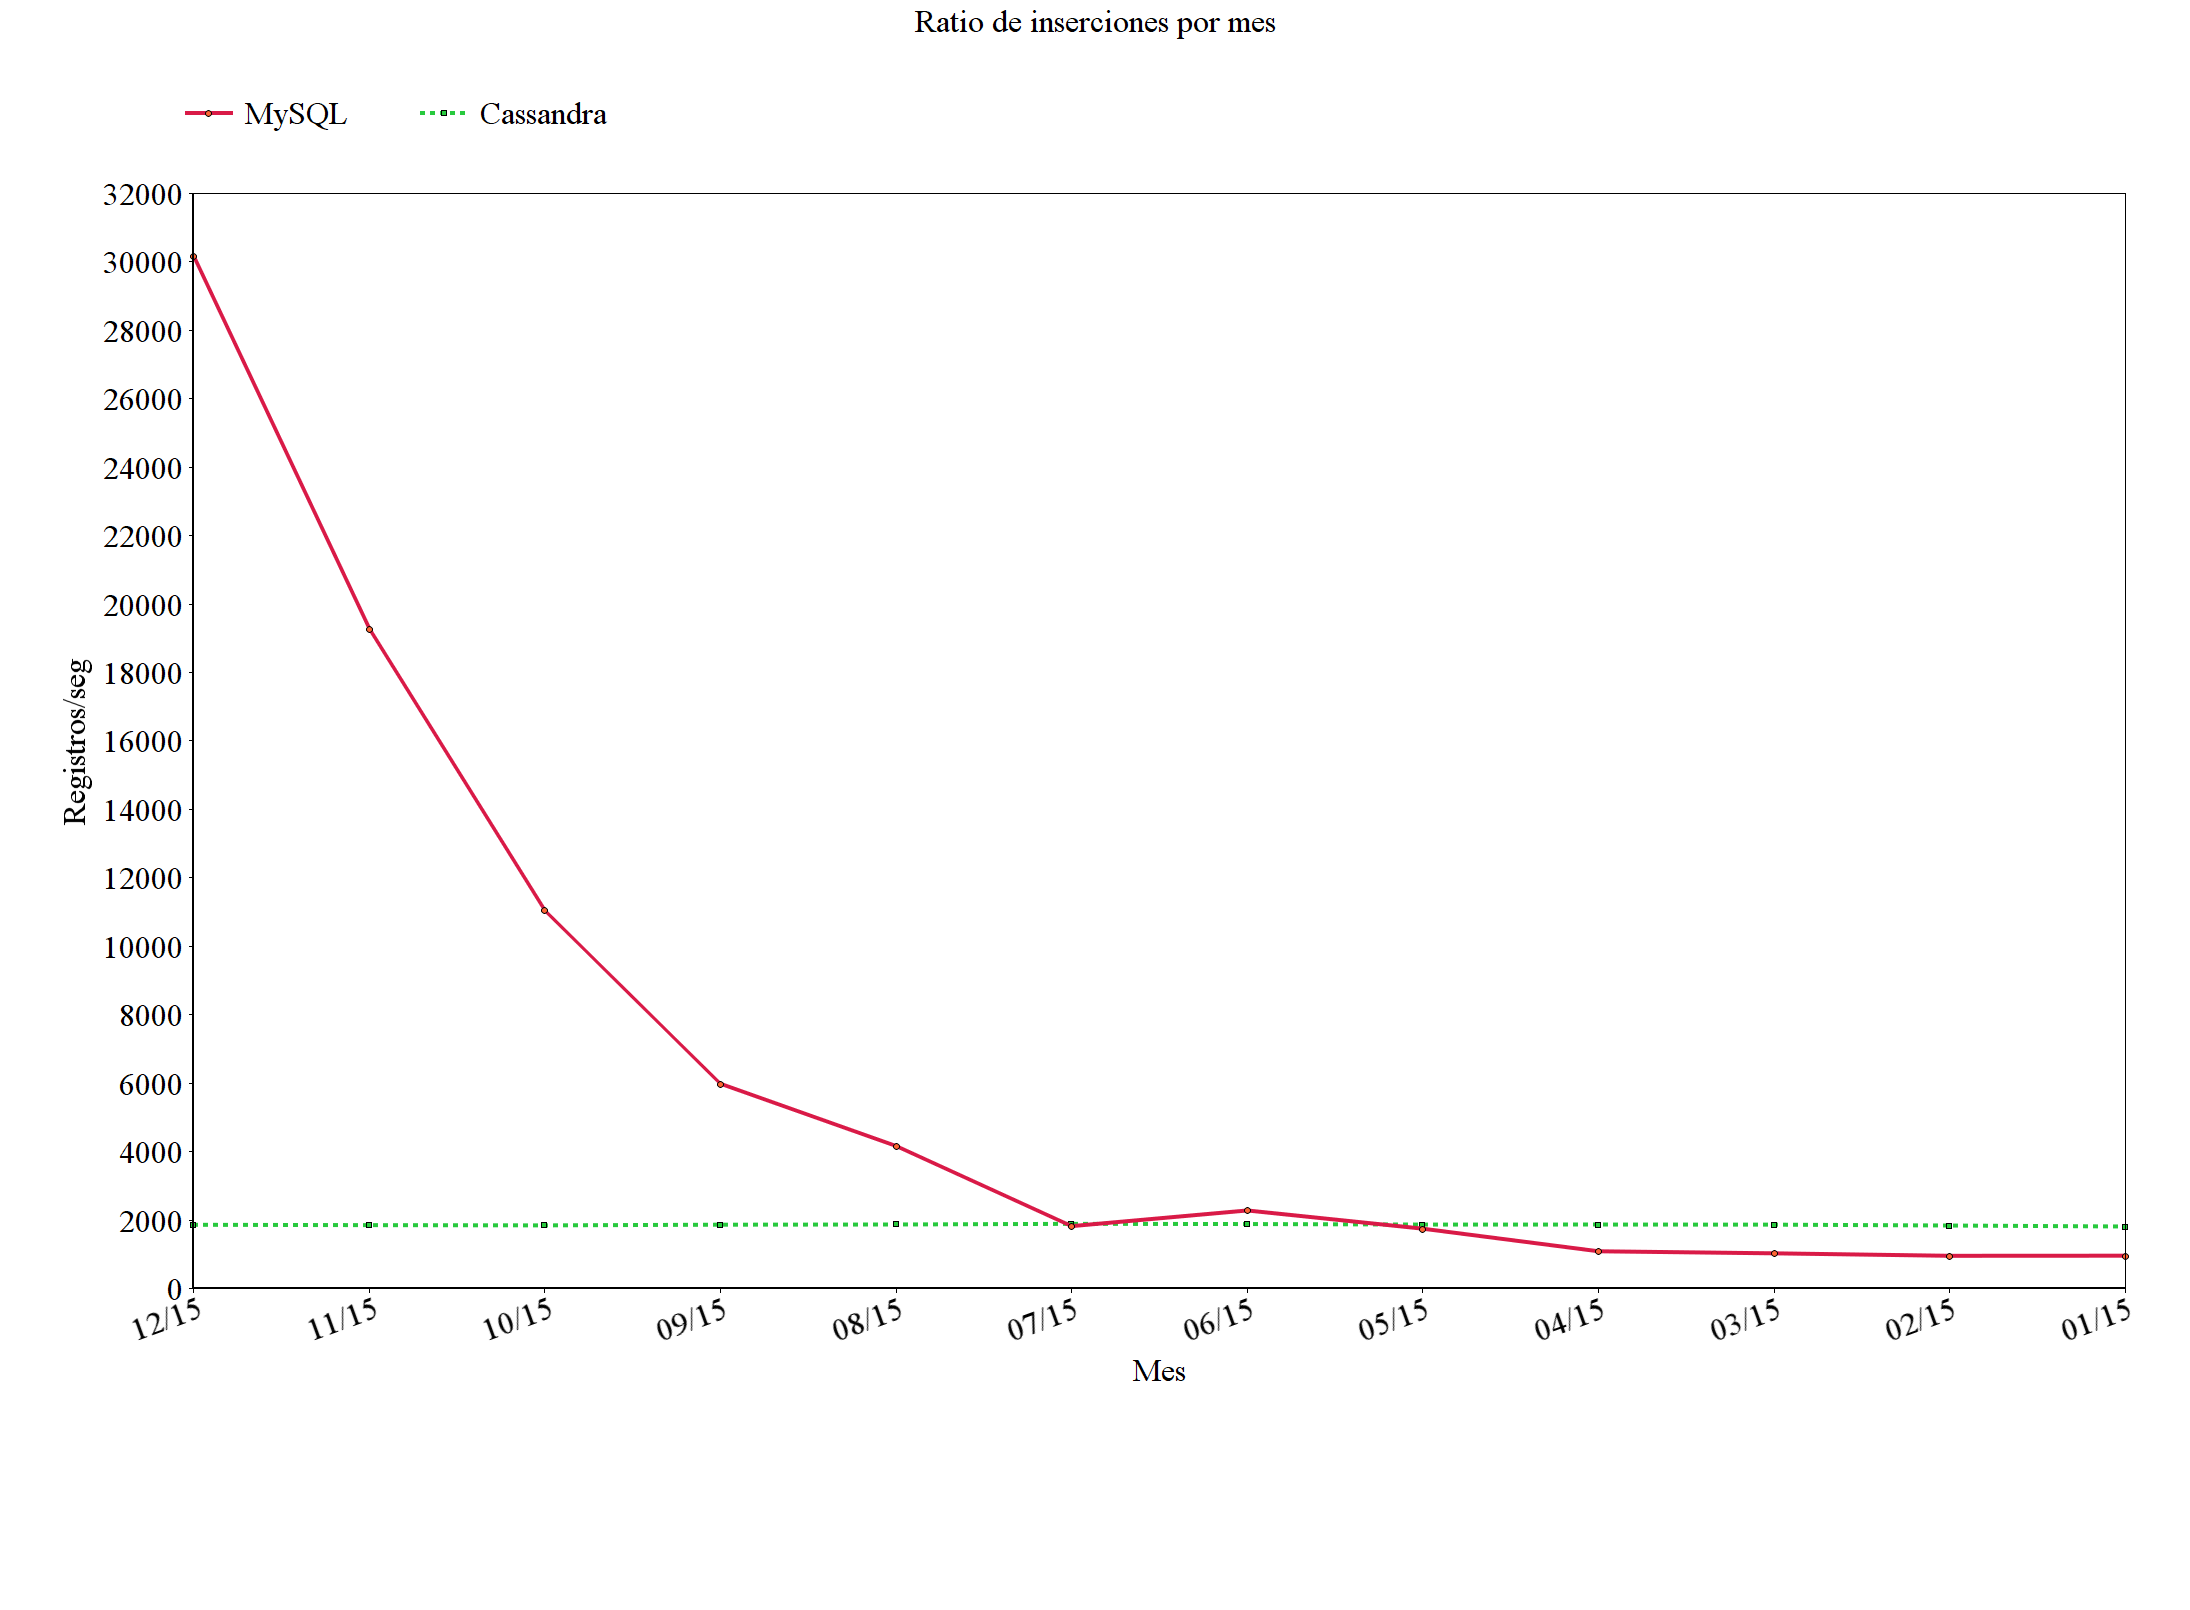
\includegraphics[width=1\textwidth]{Ilustraciones/registrosPorSeg.png}
 \end{figure}
 
\subsection{Consultas de Lectura}
 
 \begin{figure}[h]
 	\centering
 	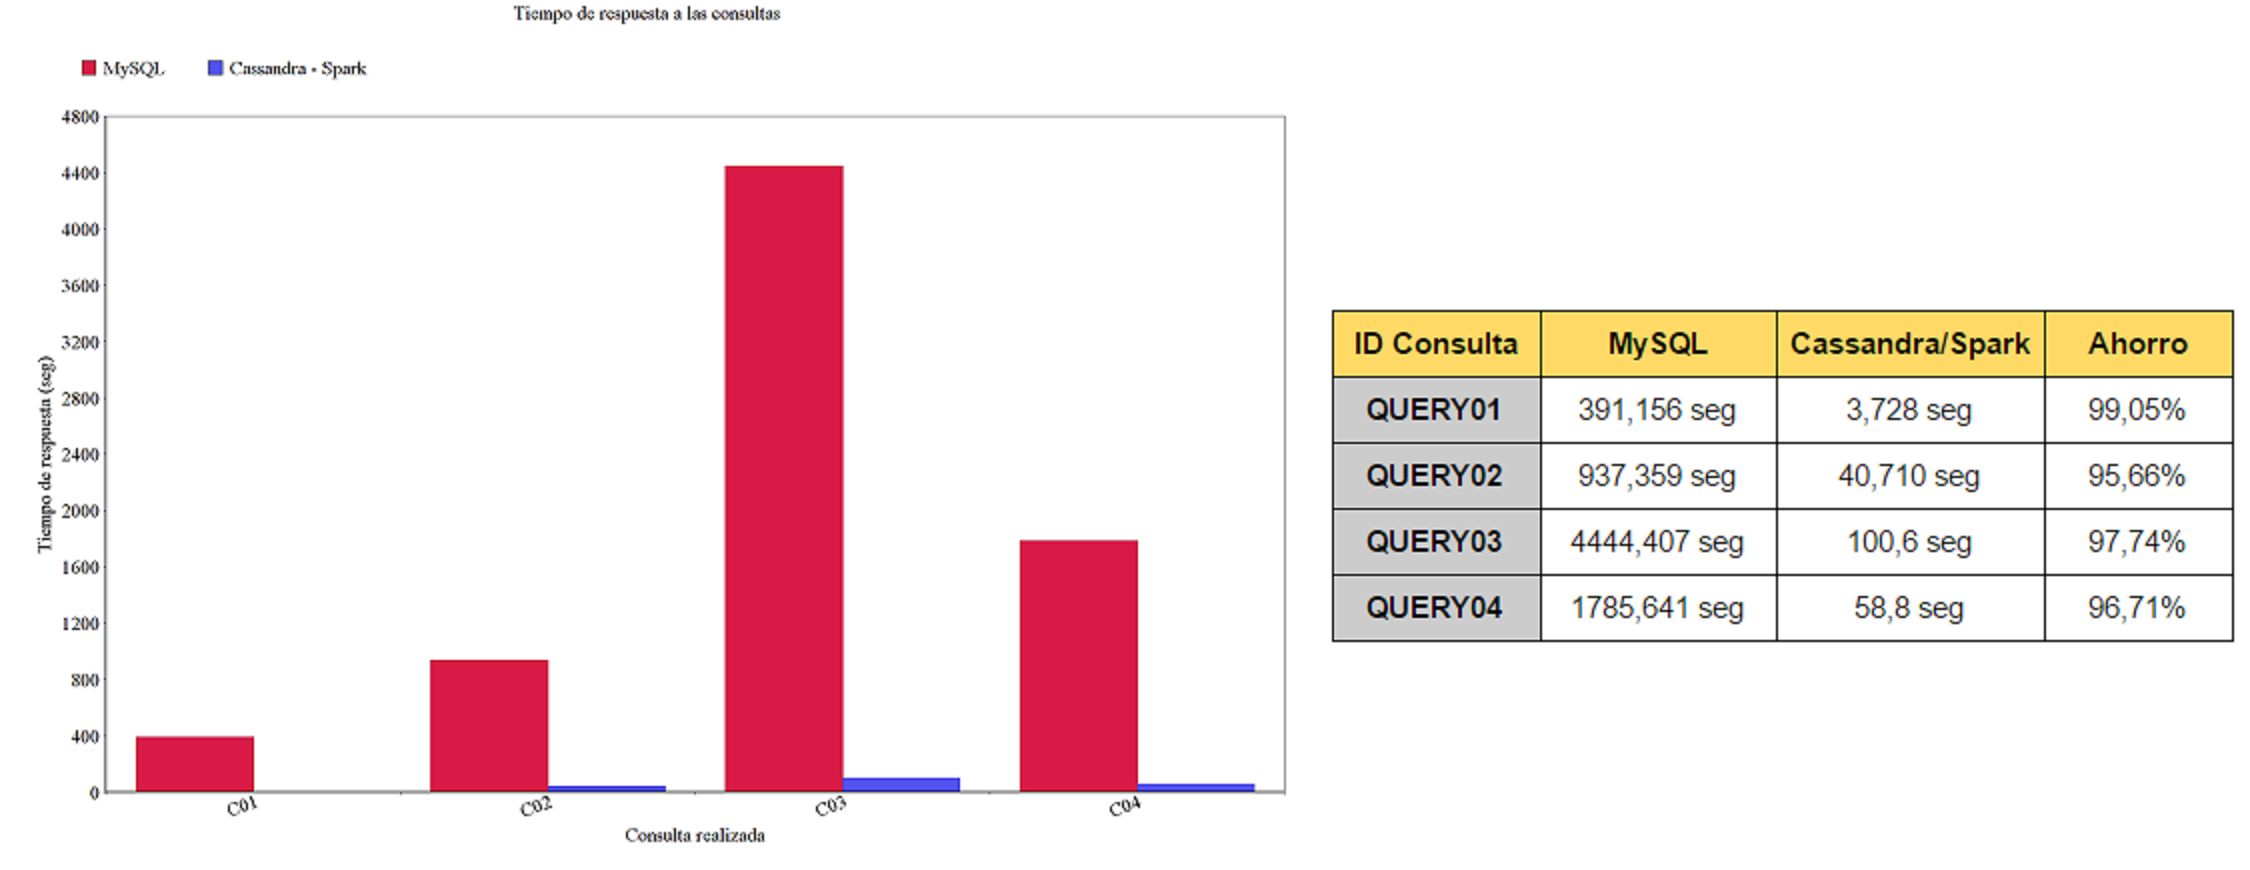
\includegraphics[width=1\textwidth]{Ilustraciones/TiempoRespuestaConsultas.png}
 \end{figure}
 
 


